\section{Urbanismo, urbanización y urbe}

\subsection{Definiciones generales}

Lo más lógico a la hora de recurrir a definiciones es la utilización del diccionario y a un proceso
de semiosis etimológica. A partir de esta semiosis es que se hace necesario identificar los
conceptos de urbe, urbanismos, urbanización, ciudad, barrio, por nombrar algunos.

Se tiende a diferenciar lo urbano de lo rural, considerando al primero relativo a la
urbe, es decir, ciudades altamente pobladas con una infraestructura servil a la interrelación de
determinados servicios sociales y las condiciones de esta infraestructura (porcentaje de calles
pavimentadas, acceso a hospitales, instituciones de educación entre otras características). Por
contra, se tiende a pensar en lo rural como lo campestre, bajos niveles de población, escaso acceso
a servicios de salud y educación, aislamiento de la ciudad. Sin embargo, la especificación sobre qué
es urbano y qué es rural es dinámica, es decir, varía acorde al tiempo y el territorio (legislación
país), pero siempre se consensúa que lo urbano es el complemento de lo rural en la distribución
espacial.

La urbanización es la ``Acción y efecto de urbanizar'', urbanizar es ``Hacer urbano, civilizar ||
Convertir un terreno en poblado abriendo calles y dotándolo de los servicios necesarios''. 
El urbanismo es el ``conjunto de conocimientos que se refieren al estudio de la creación,
desarrollo, reforma y progreso de los poblados en orden a las necesidades de la vida urbana''.

Al momento de concebir la función civilizadora de la urbanización se comprende que 
converge con otras disciplinas tales como la ingeniería civil, la arquitectura, la psicología, el
derecho, la lingüística, la antropología, la sociología, la semiótica y la política por nombrar algunas
\cite{Wkur}, puesto que el acto de civilizar es una tarea netamente cultural y que está sujeta a las
necesidades de la sociedad en determinado contexto. Está estrechamente relacionado con el desarrollo
y evolución del concepción de derechos de una determinada cultura, puesto que es el entendimiento y
satisfacción de estos derechos el que es determinante en la infraestructura urbana para asegurar el
bienestar de la población. Incluso, el concepto de urbanización y las métricas que determinan si un
espacio urbano cumple con las condiciones para considerarse como tal, más allá de la cantidad de
personas que conforman el poblado, van de la mano con el estudio de las condiciones
socio-económico-ambientales que tienen lugar dentro del mismo.


Acorde a lo anterior, se aprecia una marcada diferencia entre los conceptos de urbanismo y
urbanización, el urbanismo se dedica a la planificación del suelo interlocal, incluso abarcando
ámbitos de carácter rural, se dedica a la ordenación de las ciudades y del territorio.
La urbanización, por contra, se enfoca en los procesos constructivos, más
no con la ordenación urbana. Se podría hacer entendible esta diferencia abocando a que la
urbanización es la práctica del urbanismo.



\subsection{Definiciones de acuerdo a la legislación chilena}
\begin{quote}
\flushright{
\textit{
``Es evidente que la legislación urbana no puede seguir ignorando los derechos de las personas a tener
un lugar donde vivir con seguridad y dignidad. 
El impacto crítico de la desigualdad en la tenencia de la tierra en el entorno urbano exige que la
población urbana pobre tenga acceso a la información técnica necesaria para negociar mejor sus
inquietudes con los funcionarios públicos''
}
}

\textbf{Sonia Pereira}, Equidad en el acceso al suelo  para la población urbana pobre. 1997

\end{quote}

Las definiciones varían de un país a otro, sin ir más lejos y luego de las definiciones generales en
el capítulo anterior, se pueden identificar una serie de especificaciones frente a conceptos como la
urbanización, que también se entiende como el conjunto de viviendas situadas generalmente en un
antiguo medio rural junto a otras poblaciones\cite{Wkuv}.
En el plano nacional, de acuerdo a la Ordenanza General de Urbanismo y Construcciones, en el Capítulo 2: De las
Normas de Urbanización, artículo 2.2.1, se especifica lo siguiente:

\begin{quote}
``Se entiende por
urbanización la ejecución o ampliación de obras de infraestructura y ornato señaladas en el artículo
134 de la Ley General de Urbanismo y Construcciones, que se ejecutan en el espacio público
existente, al interior de un predio en las vías contempladas en un proyecto de loteo, o en el área
del predio que estuviere afectada a la utilidad pública por el Instrumento de planificación
Territorial respectivo.

La urbanización comprende dos tipos de gestión:
\begin{enumerate}
  \item La ejecución de obras de urbanización al interior de un predio por parte de su propietario.
  \item Le ejecución de obras de urbanización en el espacio público, por parte de los municipios u otros
        organismos públicos. ''
\end{enumerate}

En la misma Ordenanza General de Urbanismo y Construcciones, en el Título 1 ``Disposiciones
Generales'', Capítulo 1 ``Normas de competencia y definiciones'', Artículo 1.1.2; se pueden
encontrar las siguientes definiciones:

\begin{description}
  \item[Área rural:] territorio ubicado fuera del límite urbano.
  \item[Área urbana:] superficie del territorio ubicada al interior del límite urbano, destinada al
  desarrollo armónico de los centros poblados y sus actividades existentes y proyectadas por el
  instrumento de planificación territorial.
  \item[Área de extensión urbana:] superficie del territorio ubicada al interior del límite urbano,
  destinada al crecimiento urbano proyectada por el plan regulador intercomunal.
  \item[Barrio:] área habitacional, industrial, comercial o mixta que forma parte de una ciudad,
  compuesta generalmente de un grupo de manzanas con características similares.
  \item[Límite urbano:] línea imaginaria que delimita las áreas urbanas y de extensión urbana
  establecidas en los instrumentos de planificación territorial, diferenciándolos del resto del área
  comunal.
  \item[Límite de extensión urbana:] línea imaginaria que determina la superficie máxima destinada al
  crecimiento urbano proyectado por el plan regulador intercomunal.
  \item[Lote:] superficie de terreno continua resultante del proceso de división y urbanización del
  suelo, o de modificaciones, anexiones o sustracciones de la misma.
  \item[Sistema de Información Geográfica:] herramienta informática que permite el manejo de
  información planimétrica georeferenciada en interacción con bases de datos asociadas.
  \item[Urbanizar:] ejecutar, ampliar o modificar cualquiera de las obras señaladas en el artículo
  134 de la Ley General de Urbanismo y Construcciones que correspondan según el caso, en el espacio
  público o en el contemplado con tal destino en el respectivo instrumento de Planificación
  Territorial o en un proyecto de loteo.
\end{description}
\end{quote}

El Artículo 134 del párrafo 4$^{o}$ de la Ley General de Urbanismo y Construcciones dice lo
siguiente:

\begin{quote}
Para urbanizar un terreno, el           
propietario del mismo deberá ejecutar, a su costa, el      
pavimento de las calles y pasajes, las plantaciones y      
obras de ornato, las instalaciones sanitarias y            
energéticas, con sus obras de alimentación y desagües de 
aguas servidas y de aguas lluvias, y las obras de 
defensa y de servicio del terreno.

    Sin embargo, cuando las obras de alimentación y 
    desagüe que deban ejecutarse beneficien también a otros 
    propietarios, el servicio respectivo determinará el pago 
    proporcional que corresponda al propietario en estas 
    obras, en la forma que determine la Ordenanza General.
    
        Las plantaciones y obras de ornato deberán ser         
        aprobadas y recibidas por la Dirección de Obras            
        Municipales respectiva.                                    
\end{quote}

Mayores especificaciones sobre la legislación chilena relativa a materias de urbanismo, como el Plan
de Desarrollo Urbanístico Regional, plan Regulador y otros mecanismos provistos por el Ministerio de
Vivienda y Urbanismo o el Ministerio de Obras Públicas corresponden a una investigación posterior.

\subsubsection{Lo urbano y lo rural acorde al Censo chileno}

El censo es el padrón de la población nacional, para que sea llevado a cabo se define una división
geográfica censal que debe ser operativa, homogenea, representativa y de codificación única. Esta
estructura queda representada en la figura~\ref{censo}, que nos entrega una rápida descripción de la
división territorial chilena. 

\begin{figure}
  \centering
  \caption{División territorial censal}
  \label{censo}
  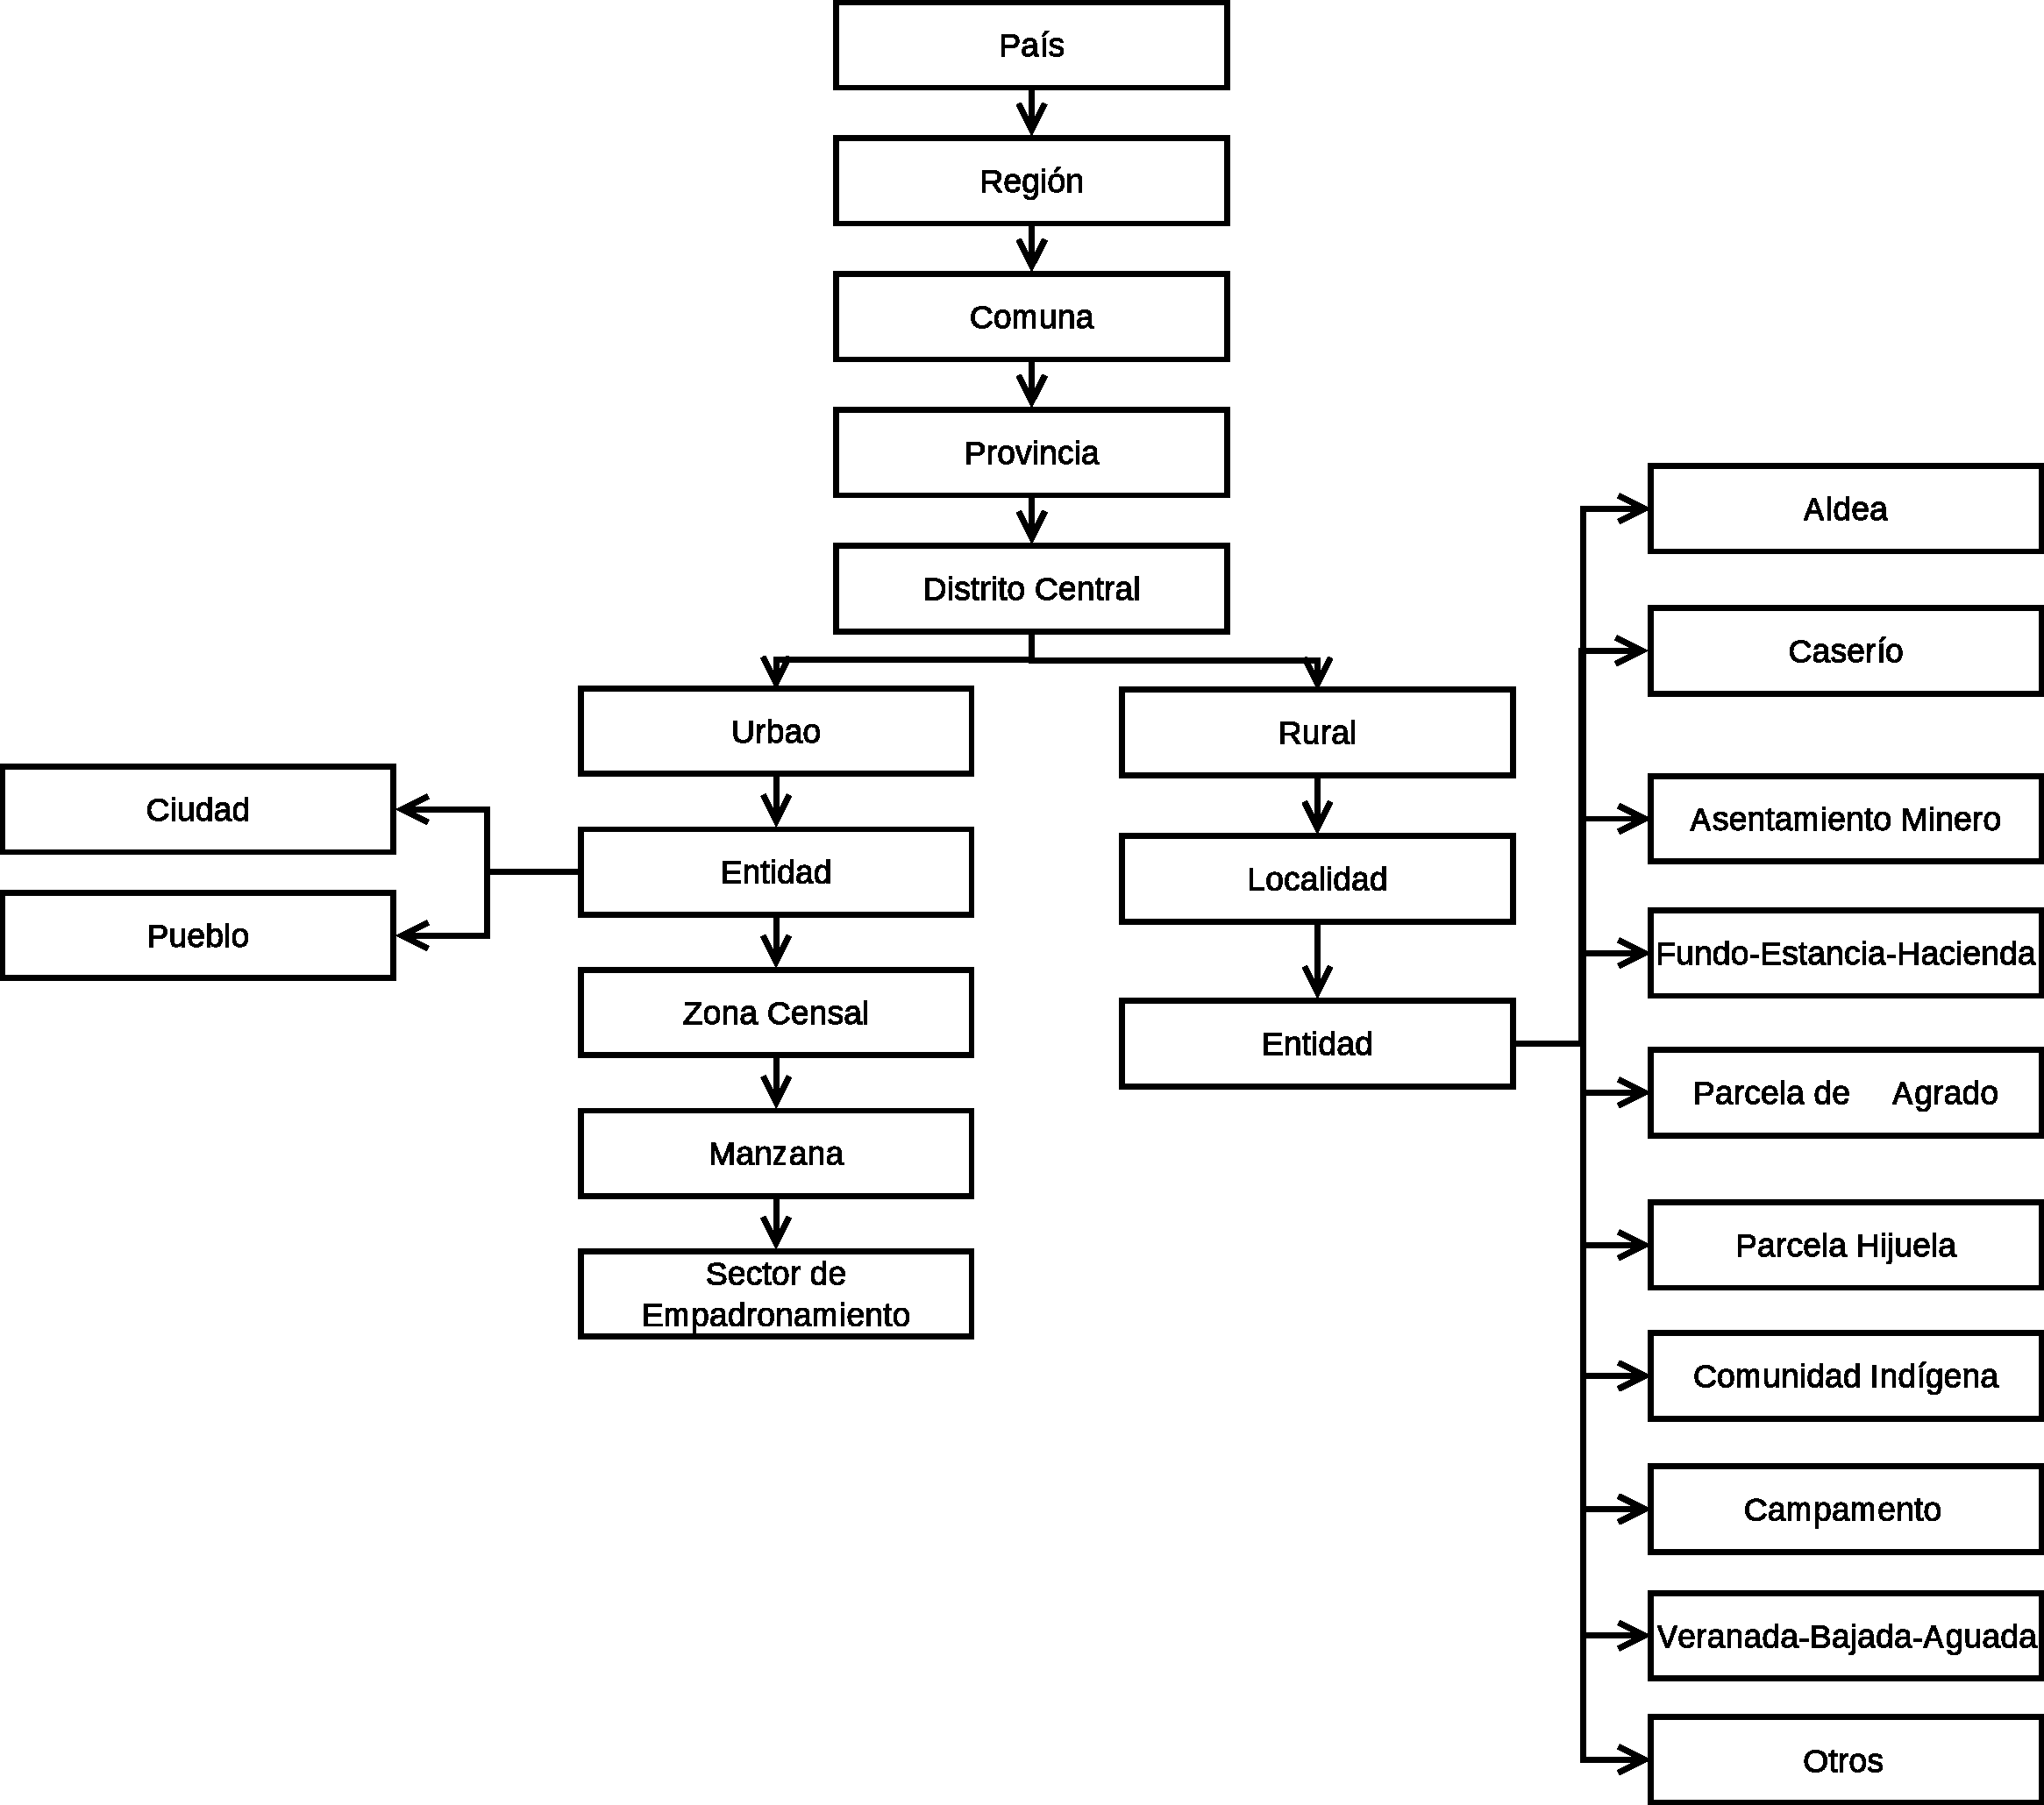
\includegraphics[scale=0.25]{censo}
\end{figure}

El INE ha definido la conformación del distrito censal, que es la unidad
geográfica que subdivide a la comuna con fines censales en dos áreas: (1) área urbana y (2) área
rural, estas áreas son dicotómicas, es decir, lo urbano es lo contrario a lo rural. Sin embargo,
como ya se ha mencionado con anterioridad en este documento, los conceptos de urbano y rural varían
de acuerdo al tiempo. De este modo es como podemos distinguir las siguientes definiciones que ha
hecho el INE para los distintos censos desde 1960 hasta el 2002 relativas a lo urbano:

\begin{description}
  \item[Censo 1960:] Todas las poblaciones del país con características urbanas (ciudades, pueblos,
  aldeas, minerales, salitreras y otros centros poblados con dichas características, como bases
  aereas, campamentos, etc) ya sean concentradas con algunas calles pavimentadas o con algunos
  servicios de utilidad pública.
  \item[Censo 1970:] Área que presenta un límite mínimo de 40 viviendas continuas o agrupadas, con
  definición preestablecida de calles y que además cuenta con alguno de los siguientes servicios:
  carabineros, correo, luz eléctrica, agua potable, alcantarillado, comercio establecido, escuela.
  \item[Censo 1982:] Todo lugar habitado que presenta rasgos de urbanización, al menos incipiente,
  idependientemente de la actividad que desarrollan sus habitantes, y que cuenta con un mínimo de 60
  viviendas agrupadas y contiguas, siempre que su población no sea inferior a 301 habitantes.
  Excepciones: aeropuertos, centros de turismo y esparcimiento y caseríos cordilleranos altiplánicos
  del Norte Grande que no alcancen los montos mínimos de población y vivienda establecidos.
  \item[Censo 1992:] Conjunto de viviendas concentradas con más de 2.000 habitantes , o entre los
  1.001 y 2.000 habitantes, con el 50\% o más de su población económicamente activa dedicadas a las
  actividades secundarias y/o terciarias. Excepcionalmente, los centros que cumplen funciones de
  turismo y recreación con más de 250 viviendas concentradas y que no alcanzan el requisito de
  población que se consideran urbanos.
  \item[Censo 2002:] Conjunto de viviendas concentradas con más de 2.000 habitantes, o entre 1.001 y
  2.000 habitanes, con el 50\% o más de su población económicamente activa dedicadas a las
  actividades secundarias y/o terciarias. Excepcionalmente los centros que cumplen funciones de
  turismo y recreación con más de 250 viviendas concentradas y que no alcancen el requisito de
  población se consideran urbanos.
\end{description}
